\documentclass[final, 3p, 11pt]{elsarticle}

% Packages
\usepackage{lmodern}
\usepackage[T1]{fontenc}
\usepackage{amsmath}
\usepackage{graphicx}
\usepackage{booktabs}
\usepackage{multicol}
\usepackage[version=4]{mhchem}
\usepackage{subcaption}
\usepackage{listings} % For code
\usepackage{float}

\usepackage[numbers]{natbib}
\bibliographystyle{plainnat}

\setlength{\parskip}{1em}
\setlength{\parindent}{0pt}

% Python code style settings
\lstset{
  basicstyle=\ttfamily\footnotesize,  % Code font
  numbers=left,                       % Line numbers
  numberstyle=\tiny,                  % Line number style
  numbersep=5pt,                      % Line number spacing
  language=Python,                    % Python syntax highlighting
}

\usepackage[hidelinks]{hyperref}

% Begin document
\begin{document}
\begin{frontmatter}

% Title Page

\title{4TR3 - Capstone Midterm Report\\}
\title{Non-intrusive Testing of Liquid Culture Medium using Online NIR Spectroscopy and Machine Learning for Qualitative Analysis}

\author[1]{Benjamin Samuel\fnref{cor3}}
\author[1]{Connor Reintjes\fnref{cor1,cor2}}
\author[1]{Paola Gonz\'alez P\'erez\fnref{cor2}}
\author[1]{Shiza Hassan\fnref{cor3}}
\author[1]{\\Dr. Amin Reza Rajabzadeh\fnref{cor4}} % Supervisor as corref

\fntext[cor1]{Conceptualization} % Custom footnote for dry-lab-1
\fntext[cor2]{Validation \& Software} % Custom footnote for dry-lab-2
\fntext[cor3]{Investigation \& Methodology} % Custom footnote for wet-lab
\fntext[cor4]{Principle Investigator \& Capstone Supervisor} % Custom text for Supervisor

\affiliation[1]{organization={McMaster University, W. Booth School of Engineering Practice and Technology}, city={Hamilton, ON.}, country={Canada}}

\begin{abstract}
Insufficient quality assurance is a major expense associated with laboractories that an result in contamination, poor sample integrity, and lead to lost time due to repetitive sample testing. To ameliorate these issues, NIR spectroscopy has been combined with machine learning in this approach to qualitatively analyze the composition of liquid cultures in a non-intrusive and online manner. This will allow laboratories to save time by identifying contamination as soon as it happens and proceeding accordingly, as opposed to finding out after a full protocol has been performed. The method to achieve this involved creating a handheld casing to house the NIR which would take spectra of the sample and pass it to a machine learning model that would then identify whether the sample is in a normal or contaminated state. In phase 1 of the experiment, the NIR housing was built and initial testing was conducted for both contaminated and non-contaminated states, with the contaminant being Lactobacillus rhamnosus. The results achieved indicate that the NIR was able to differentiate between contaminated and non$-$contaminated samples. To analyze these readings a 1D$-$CNN model will be trained with the data collected thus far in the second phase of the experiment. Moving forward, further testing will be performed using quartz cuvettes to achieve more accurate and precise results as well as plating of bacteria to generate a standard curve to achieve quantitative results. 

\end{abstract}

\begin{keyword}
Bioprocess Monitoring \sep Machine Learning \sep Near$-$Infared Spectroscopy (NIR) \sep 1D Convolutional Neural Network (1D$-$CNN) \sep Qualitative Analysis
\end{keyword}

\end{frontmatter}

% Introduction

\section{Materials and Methods}

\subsection{NIR Housing Design}
The custom housing for the NIR was 3D printed using a Bambu Lab P1S. The majority of the housing was constructed using Acrylonitrile butadiene (ABS) filament however, the cuvette holder was printed using polylactic acid (PLA) filament. The sides and bottom of the cuvette holder were printed in black PLA, while the background was printed in white PLA to increase reflectance. 

This white PLA background was not as reflective as originally theorized, so the use of teflon (PTFE) was considered. A high-reflectance PTFE sheet with 3M Adhesive backing was purchased from ThorLabs. This sheet has a reflectance $( >90\%)$ in the UV spectrum, and is one factor attributed to improving the SNR within the scans.

\subsection{Data Augmentation}
Due to the limited number of samples that were able to be collected, the data was augmented for the sake of training. Different data augmentation methods were explored to best fit our use case. Factors such as simplicity, and reducing the risks of overfitting were considered. The use of subsampling was determined to be the optimal method and was applied to future data collection.

\subsubsection{Pipeline Subsampling}
The data augmentation pipeline that was created is based on a type of subsampling called cyclic subsampling. Cyclic subsampling divides the dataset into non-overlapping subsets using an offset starting index and a set interval. This method has a few key features that make it optimal for this dataset when compared to other methods like temporal subsampling with sliding windows or random sampling. Since the interval remains the same across all subsamples, the temporal order of the dataset can be maintained when training a neural network. The non-overlapping sub-samples have a lower redundancy within the datasets compared to other methods, which will help prevent overfitting. The improved diversity would also allow the model to account for variations in starting time or time accumulation from scan duration.

\subsubsection{Subsampling Considerations}
Using cyclic subsampling had some major considerations that changed future data collection. The subsample interval would have to be large enough to prevent redundancy, while also remaining small enough to not create a large margin of error within the model. The frequency of scans would also have to be high enough to prevent the offset time points from approaching the cycle interval. Due to these considerations, our scanning frequency was changed to 60 second intervals. Our default augmentation parameters were set at a 60 second offset with a 15 minute (900 second) cycle interval with 3 subsamples per dataset. 

\subsection{One-Dimensional Convolutional Neural Network}
The classification of near-infrared (NIR) spectra to determine the contamination state of liquid media was performed with a one-dimensional convolutional neural network (1D-CNN). This neural network model uses the Keras library with Tensorflow as the backend. The use of Keras facilitates the modelling of the CNN due to its intuitive and user-friendly interface (Keras Team, n.d.). The Tensorflow backend allows for accelerated training when used with GPU (AceCloud Team, 2024). It also enables a detailed visualization through Tensorboard. Their combination results in a flexible model with easily customizable variables, like the layers and optimizers, along with shorter training times

\subsubsection{Model Architecture}
The model consists of two Conv1D layers, with 64 and 32 filters respectively. These filters allow for the extraction of significant features in the input data (Nisha \& Meeral, 2020). These features set the parameters that will be learned throughout training. To avoid overfitting and reduce the dimensionality of these parameters, MazPooling1D layers and Dropout layers are implemented after the Conv1D layers. The activation function, or function that transforms the input of a node into an output of that node, is a key component of a neural network. The model uses the Rectified Linear Unit (ReLU) function as the activation function, which only outputs non-negative outputs or zeros (Brownlee, 2019). This is commonly used in CNNs due to its ease of training and superior performance. A final dense layer is implemented with a sigmoidal activation function. This function outputs a probability score between 0 and 1 to determine the contamination state of the sample: 0 for non-contaminated and 1 for contaminated (Saeed, 2021).

\subsubsection{Optimizer and Loss Function}
Optimizers are functions responsible for adjusting the parameters as training progresses (EITCA Academy, 2023). This is done to reduce the loss function, a mathematical quantification of the error margin between the prediction and the ground truth. The Adam algorithm was chosen as the optimizer. This follows a stochastic gradient descent based on adaptive estimation and regulated by the learning rate (Keras Team, n.d.). It allows for the model to reach an optimal point faster without taking large learning steps that could lead to skipping key information during training. The learning rate was set to 0.0005 to avoid reaching a convergence between the ground truth and prediction too early during training.

\begin{align*}
  L = -\frac{1}{N} \sum_{i=1}^{N} \left[y_i \cdot \log(p(y_i)) + (1 - y_i) \cdot \log(1 - p(y_i)) \right]
  \label{eq:cross_entropy}
\end{align*}

The binary cross-entropy loss function was used in the model due to the binary classification nature of the project. This loss function is defined as where y is the label (1 for contaminated and 0 for non-contaminated) and $p(y)$ is the predicted probability of the point being contaminated for all N points. Binary cross-entropy quantifies the differences between the logarithmic probability distributions and penalizes inaccurate predictions which helps assess the model’s prediction confidence.


\subsubsection{Training Parameters}
Since the small size of the training dataset represents a major problem for the accuracy of the model, the number of epochs, or cycles that the entire dataset passes through the algorithm during training, was adjusted to offset this limitation. The model was trained with 15 epochs to reduce the risk of overfitting, and an early stopping callback was included to stop the training process once the model showed no further improvement after each epoch. To ensure an efficient use of the limited dataset for both training and validation, cross-validation was implemented. This allowed for both the training and validation batch size to be 18, the total dataset size.

\section{Results}

\section{Discussion}

\section{Problems and Future Steps}

\section{Conclusion}


\section*{Acknowledgments}
Acknowledge any individuals or organizations that contributed to the research, funding bodies, and any supporting institutions.

\newpage
\bibliography{references}     % The .bib file name (without the .bib extension)

\newpage
% \section*{Appendix}

\section*{Appendix A}

% Change the figure labeling format for this appendix
\renewcommand{\thefigure}{A.\arabic{figure}}
\setcounter{figure}{0}  % Reset the figure counter

\begin{figure}[H]
    \captionsetup{justification=raggedright, singlelinecheck=false, position=above}  % Caption on top and left-justified
    \caption{Ethanol Standard Curve from Quartz Cuvette.}
    \centering
    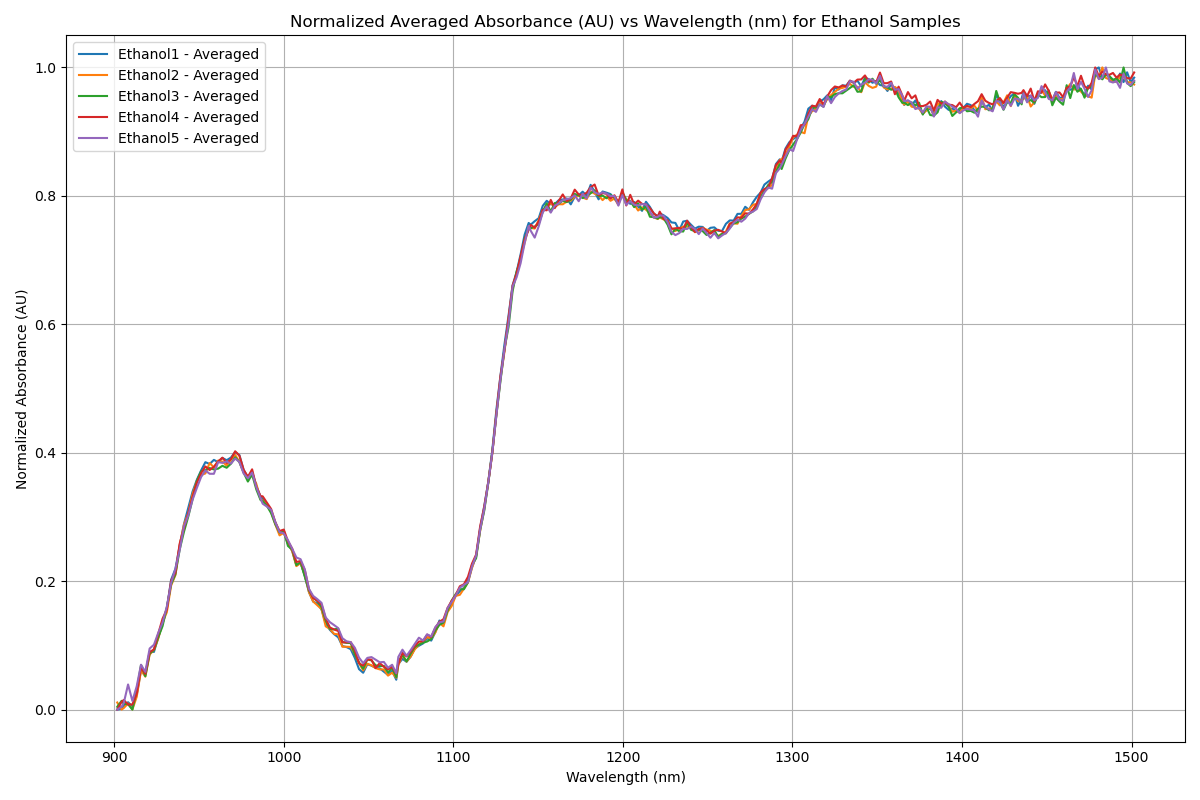
\includegraphics[width=\textwidth]{Images/Ethanol_Standard.png}
    \label{fig:appendix_ethanol_standard}
\end{figure}

\newpage
\begin{figure}[h]
  \captionsetup{justification=raggedright, singlelinecheck=false, position=above}  % Caption on top and left-justified
  \caption{Ethanol Standard Curve from Plastic Cuvette.}
  \centering
  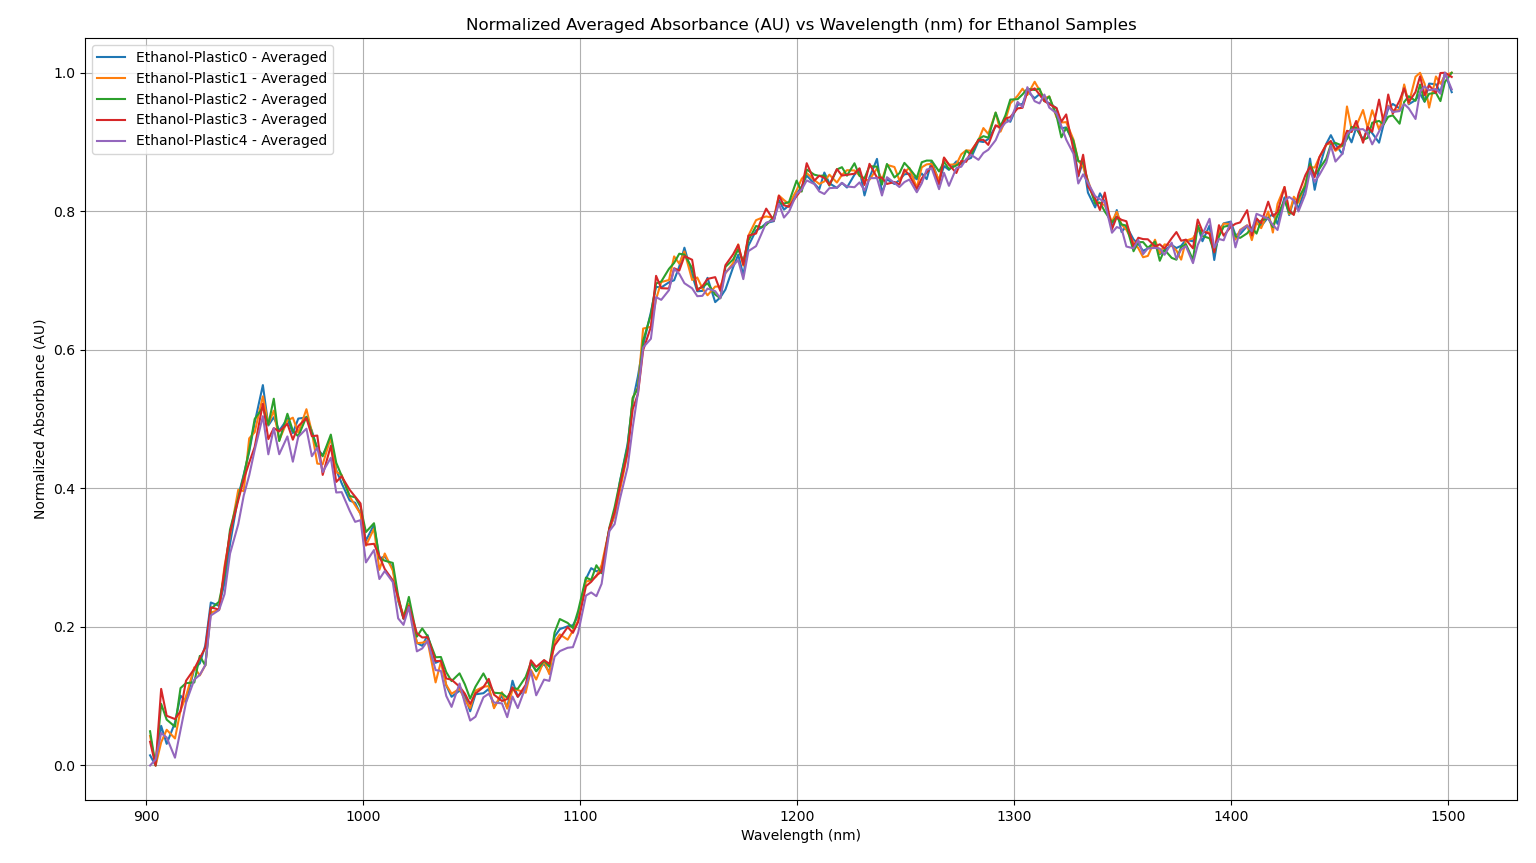
\includegraphics[width=\textwidth]{Images/Ethanol-Plastic_Standard.png}  % Replace with your image file
  \label{fig:appendix_ethanol_plastic}
\end{figure}

% End document
\end{document}
